\bbs{Puppy}

The canine-inspired robot Puppy was designed to prove the feasibility of using
pneumatic muscles for actuating a quadruped robot. The design focuses on 
imitating the musculoskeletal parameters of an adult greyhound 
\cite{PuppyDesign}. This work is motivated by extensions and potential
improvements to a control method developed by Alex Hunt in
\cite{HuntPhDThesis} and \cite{HuntHindLegWalking}. Among other areas identified
for improvement and future work, the Hunt thesis in particular cites accurate torque
profiles as a key improvement for increasing the stability and mobility of the
robot. Related to the accurate torque profiles, the joint peak angles are
accurate to between 5 and 15 degrees, but further improving the accuracy offers
an avenue for more effective walking. One potential source of error in the
hardware system is the delay between a sensor reading, communicating the data to
an off-board computer and then communicating a command back to the robot. For the geometry of the hind legs, this error did not lead to tripping; however, with the mirrored geometry of the front legs, tripping could occur. For the hind legs, if the hip swings back too far, their is sufficient range of motion in the other joints to lift the paw off the ground to initiate swing. For the front legs, which are in a mirrored orientation from the hind legs, if the shoulder swings too far back due to a delayed control signal, the elbow and ankle joints can reach a point where their combined vertical range of motion is insufficient to lift the front paw off the ground, resulting in tripping.

\bbs{Similar Robots}

There have been multiple variations of walking robots in 2-legged and 4-legged
configurations. Canines and felines are a common inspiration for these kinds of
robots, with inspiration ranging from very low degree of freedom (single joint
per leg) robots that mimic gait timing to robots that attempt to implement
complete structural and muscular replications of dogs or cats.

\bbss{Canine Robots}

The Big Dog robot made by Boston Dynamics (along with the more recent Spot and
Spot Mini) are quadruped robots built specifically for enhanced all terrain
mobility. According to \cite{BigDog}, less than half of land terrain is
accessible to wheeled or tracked vehicles, so legged robots have the opportunity
to offer unparalleled mobility.

The robot ``Ken" is based on canine kinematics with a focus on designing for
high frequency operation. The design is focused on being lightweight while also
being biomimetic. One key design decision was the use of pneumatic muscles over
electric motors. This facilitates high speed and high frequency operation
without the typical heating and/or cooling issues. Another interesting design
decision for the Ken robot was the incorporation of a contractor muscle at the
hip. Its placement and operation shorten or lengthen the leg mechanism
independent of the flexion or extension of the leg \cite{Narioka2012}.

\bbsss{Dynamics of Canine Robots}

The dynamics of robots, even those that attempt to accurately mimic biological mechanisms, can vary significantly in performance from their biological counterparts. For example, in \cite{HindLegMorphology}, the authors found that their biomimetic leg design walked with a more efficient gate when it was oriented backwards on the robot. A biological canine's leg is oriented in a Z configuration; however, in an attempt to mimic the properties of muscles, the passive elements in the joint led to a reversed Z configuration being more efficient. This suggests that animals may have adapted gaits and stimulation patterns for redundant muscles that take better advantage of passive properties of muscles than are accommodated for in current control designs \cite{HindLegMorphology}. This work suggests that directly utilizing the passive properties or designing a controller that can adapt to its specific robot hardware could lead to a dramatic increase in efficiency.

Passive elements and the particular properties of a joint play a strong role in
the energy required to actuate the joint and the effective frequency at which the joint
can operate. In particular, \cite{Na2015} covers the design of a spring
mechanism with a high natural frequency to increase the amplitude of joint
motion during high frequency operation.

\bbss{Other Robots with Pneumatic Muscles}

% TODO(buckbaskin): insert a photo of pneumatic air muscles, one relaxed and one pressurized

In \cite{PAMApplicationSurvey}, many biorobotic applications for pneumatic
muscles are presented.
Additionally, the devices are used for medical applications where the an actuator's
inherent compliance, lighter weight and higher power output are also important. 

The Pneupard robot is a feline-inspired robot based on a cheetah's
musculoskeletal design. It is actuated using pneumatic muscles to control each 3
degree of freedom leg. To control the leg, a rules-based controller is used to switch between
states where muscle activation in an actual cat are mapped to pressures in each
muscle. This controller design was aided by taking a biomimetic approach to determining the lever
arms by which the pneumatic muscles actuate. The results showed that the simple
control system remained effective even in the face of obstacles in the robot's
path due to the compliant biomechanical design \cite{Pneupard2013}.

In \cite{Wait2014}, the authors show that a simpler controller design can be
used on a quadruped robot with biologically inspired design to achieve a highly
power dense design that walks effectively. The control approach focuses on
a high-impedance control scheme for the stance phase and a second state
that takes advantage of pneumatic actuator compliance during the swing phase.
This design does not use pneumatic muscles. Instead, the authors use pneumatic
cylinders to make the design more compact by using a single rigid pneumatic cylinder that can apply both
flexion and extension forces on a joint. 

\bbs{Braided Pneumatic Actuators}

Braided pneumatic actuators, also referred to as pneumatic artificial muscles or just pneumatic muscles, typically consist of a high pressure source, a
flexible polymer section and an exhaust valve. The muscle contracts in length
when the internal pressure is higher than the surrounding environment. During
this contraction, the muscle applies a force. One limitation of pneumatic
muscles is that they typically are unable to apply force during relaxation in
the same way a rigid pneumatic cylinder can. Instead, pneumatic muscles typically are used in
antagonistic pairs. The nonlinear nature of the pneumatic muscles combined with the
antagonistic design means that, in practice, simple linear controllers are
ineffective at accurately executing a trajectory with pneumatic muscles. This means that more complex controllers are required; however,
this also means that the controller design can be more tailored and take
advantage of the unique properties of two antagonistic nonlinear actuators.

Pneumatic muscles are less common in robotics compared with electric motors;
however,
they often result in a lighter system for controlling a joint than an
electric motor. There are trade offs to each, but pneumatic actuators offer a
higher power to weight ratio for smaller displacement at low velocity and
often are a significant improvement over electric motors at higher velocities \cite{Tavakoli2008}. These properties suggests that pneumatic muscles are well suited for applications in
biological walking robots where an increased power to weight ratio increases
the efficiency of the walking mechanism, especially at the high joint velocities
found in a stepping motion.

\bbss{Characterizing Pneumatic Muscles}

In \cite{Situm2008}, the authors analyze gas flow properties for fluidic muscles
and experimentally quantify the performance of the pneumatic muscles in an antagonistic coupling
through a pulley. One of the key results in \cite{Situm2008} motivating future work is the
demonstration for a single joint with most external factors removed. The
proportional-integral control as implemented was unable to fully correct for
errors even in a desired trajectory composed of slow steps to a constant value
where the control system had time to reach a set actuation pressure.

Pneumatic actuators are used on the Puppy robot. One of the key
benefits of using pneumatic muscles in a biologically-inspired robot design is
that the muscles have similar properties to the biological muscles that control
canines \cite{Tavakoli2008}.
During analysis of the behavior of pneumatic muscles with a static load, the muscles demonstrated a non-linear response to
changing length and the ability to apply a force. This relationship was
quantified and generalized in \cite{HuntPMuscles}. This research showed that
there is a relationship between the strain on the muscle and the pressure
required to support a fixed load that can be approximated by a shifted tangent
function. 

\begin{figure}[h!]
\centering
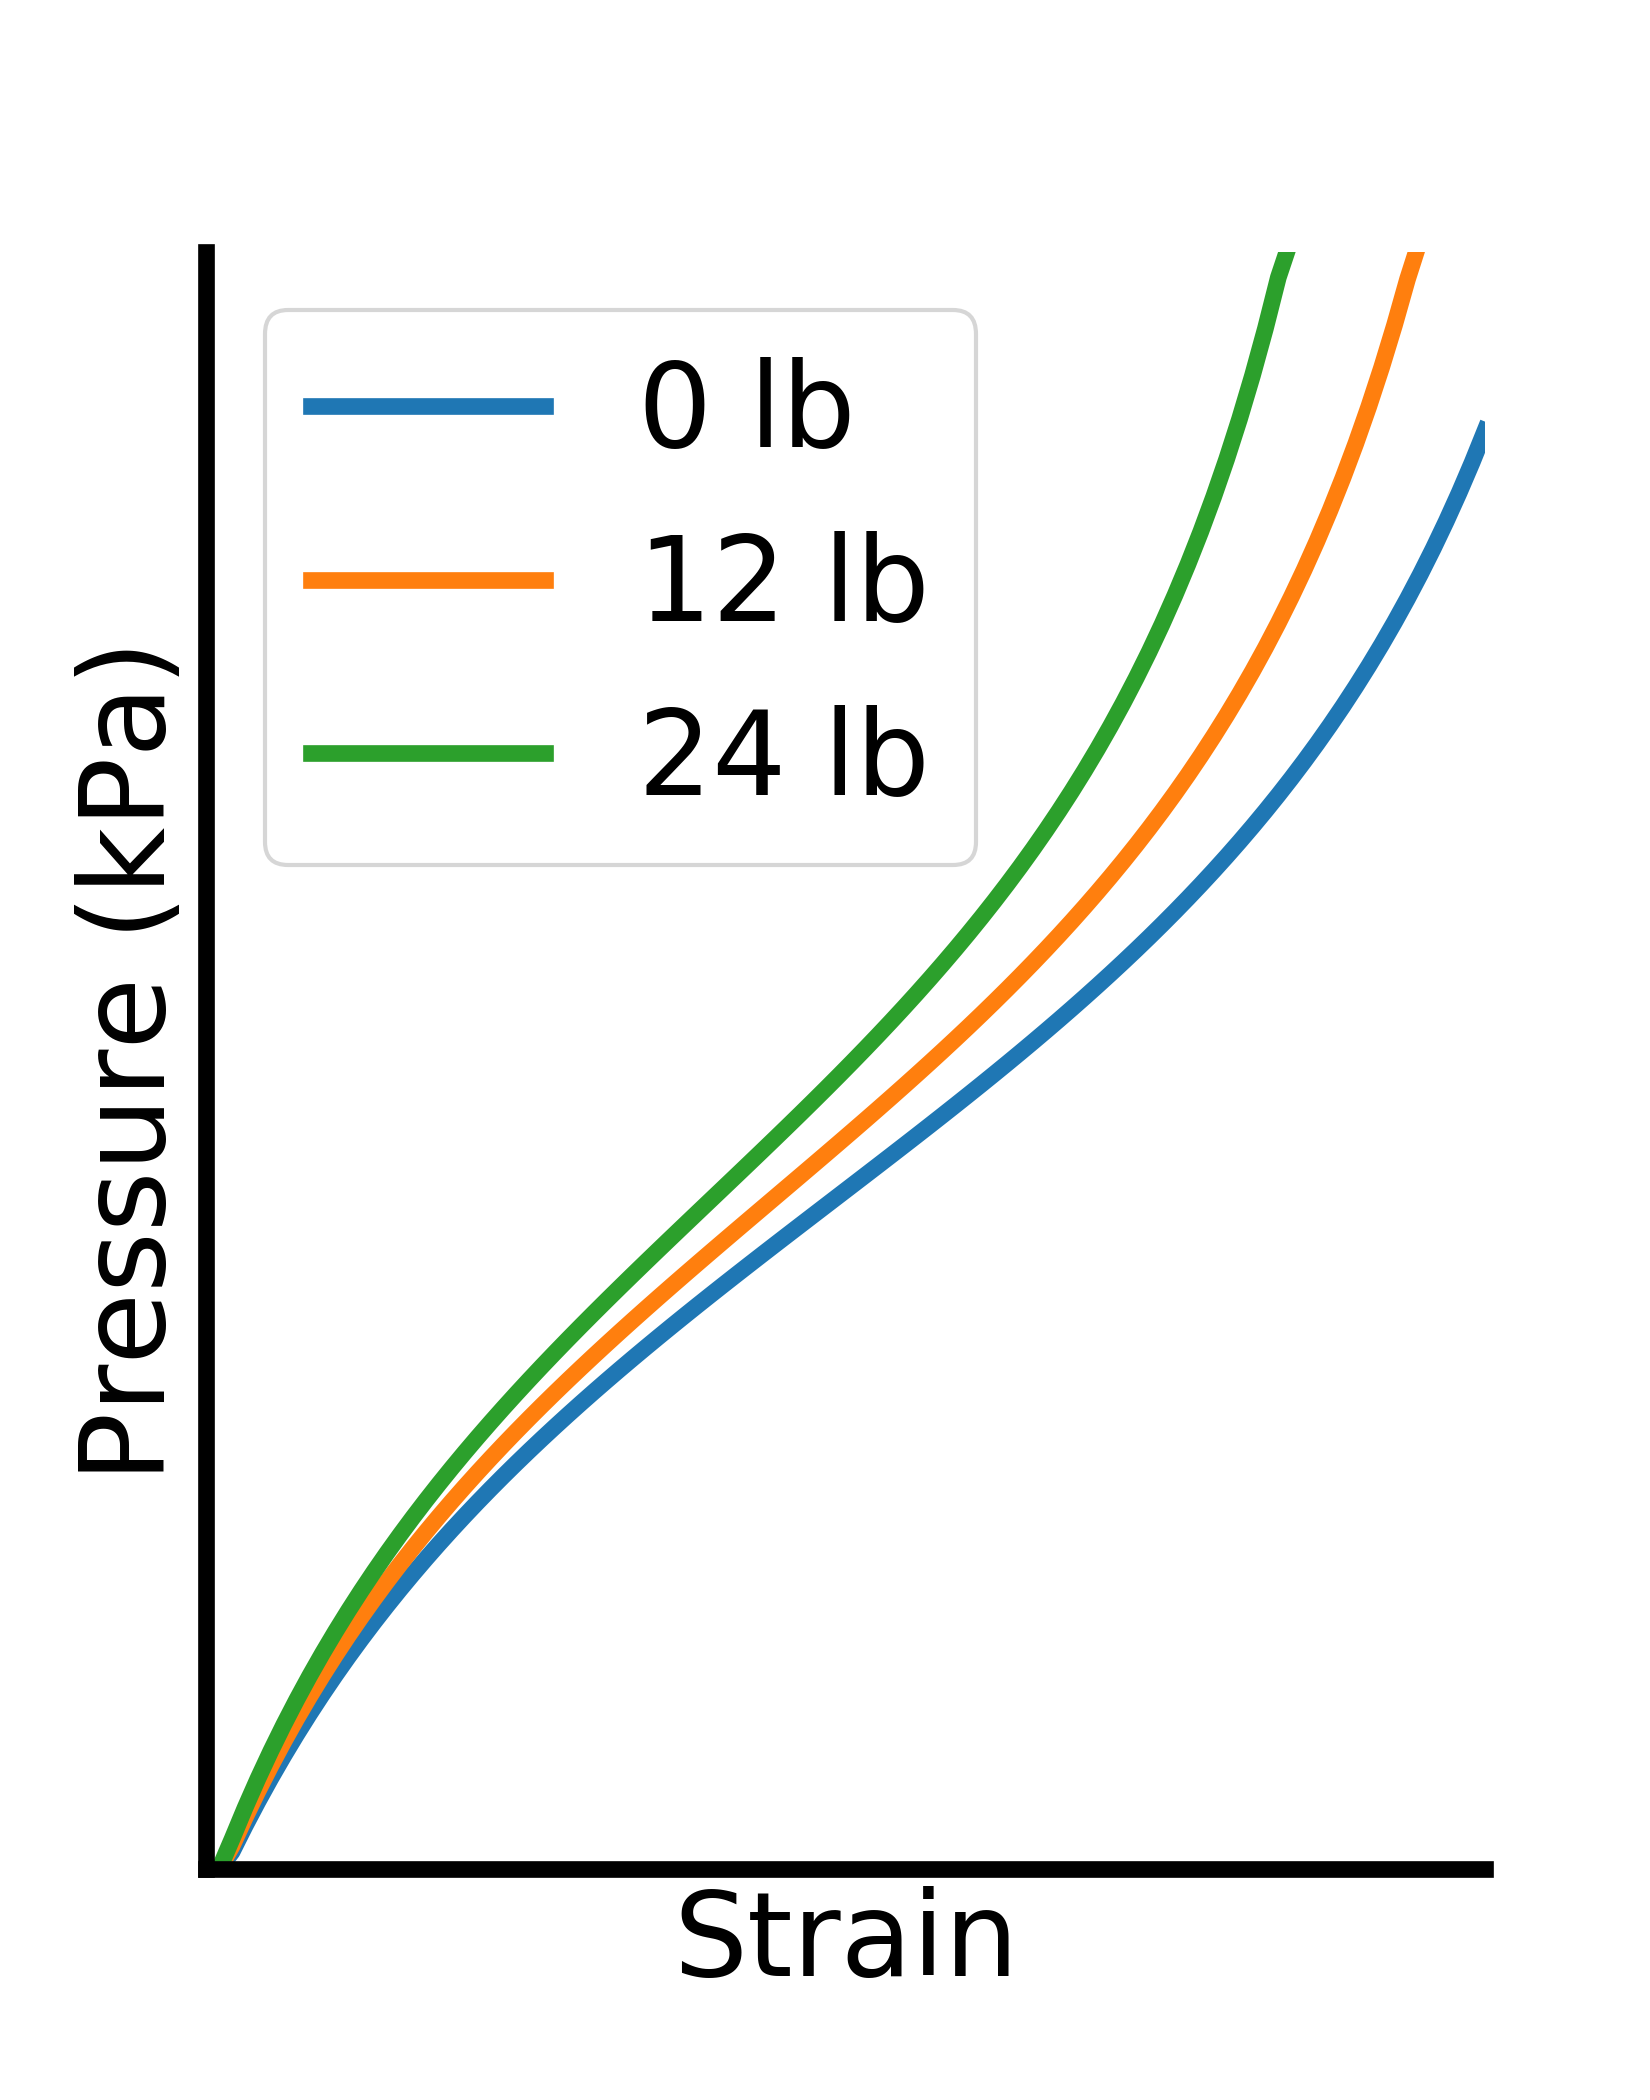
\includegraphics[width=5in]{lit_review/FigStrainPressure}
\caption{Strain/pressure relations for different applied loads}
\label{fig:StrainPressure}
\end{figure}

Using test and validation sets, the model was fit to data collected
from existing actuators on Puppy. Further, the paper goes on to show that the
model helps derive a controller for semi-static motion of joints \cite{HuntPMuscles}.

Other research with pneumatic muscles provides a model for incorporating the
dynamic properties of pneumatic actuators to allow for a more fine tuned control
process. In \cite{DynamicPMuscles}, the authors use dynamic application and
removal of load to measure the effective spring constant of the muscles and the
effective damping constant. The spring constant was shown to be correlated with
pressure, with a small constant spring effect at no pressure from the muscle
material itself. The damping coefficient was shown to be positively correlated
with pressure during contraction and weakly negatively correlated with pressure
during relaxation. The work suggests that damping comes from internal
friction in the actuator design. Additionally, the damping due to friction
effects in the input and exhaust lines is shown to be minimal compared to
internal actuator effects \cite{DynamicPMuscles}.

\bbs{Controller Design}

\bbss{Controller Theory}

Revolute joint position controllers can be treated as a function mapping the current
state (typically position, velocity and acceleration) to a torque to match the 
desired trajectory, expressed as position but often constrained to be a twice
differentiable function.

\begin{equation}
M(\theta) \ddot{\theta} + C(\theta, \dot{\theta}) \dot{\theta} + N(\theta, \dot{\theta}) = \tau
\end{equation}

In this equation, $\theta$ represents the position of the joint. $\dot{\theta}$ and $\ddot{\theta}$ represent the velocity and acceleration of the joint, respectively. $\tau$ represents the torque applied to the joint. For a single joint, $M(\theta)$ represents the mapping from the current position to the rotational inertia at the current position based on the geometry of the joint and the link it controls. In a controller for multiple joints, the link geometry may also vary based on the position of other joints. $C(\theta, \dot{\theta})$ represents the mapping from the current joint position and velocity to the damping forces on the joint. When controlling pneumatic muscles, this damping can come from external sources as well as losses from internal friction as the muscles flexes. $N(\theta, \dot{\theta})$ represents the mapping from the current joint position and velocity to conservative torque that are applied to the joint. In a robotic system, this torque can result from a weight placed on the robot or springs in the design.

If the robot starts at its desired initial state and the model of the robot is
perfectly known, the robot will exactly track the trajectory. Feedback in the 
form of sensory input is used to correct for starting error or error in the 
formulation of the exact model.

One common formulation for control is a proportional-derivative controller, 
where torque is chosen as the following:

\begin{equation}
\tau = -K_{v} \dot{e} - K_{p} e
\end{equation}

where

\begin{equation}
e = \theta - \theta_{d}
\end{equation}

In these equations, $\theta$ represents the current position of the joint and $\theta_{d}$ represents the desired position of the joint. The difference between these two values is captured in the error term $e$ and the derivative of this error with respect to time is represented as $\dot{e}$. $K_{v}$ and $K_{p}$ are gain terms that are chosen based on the system to modulate the control response to error. A higher gain increases the applied torque to counteract the error (either in position or to counteract increasing error); however, gains that are too high can destabilize the system.

The proportional-derivative (PD) controller provides a relatively simple controller design where the gain terms can be tuned such that the behavior of the overall system that is stable. On the other hand, a PD controller does not converge to
exact tracking for most real systems. In practice, an integral term is often added that accounts for steady state error to create a proportional-integral-derivative (PID) controller; however, the additional of an integral term can lead to windup or other issues.

One general method for overcoming these limitations is to use a model of the 
system to perform what is known as computed torque control, where the actuator
applies enough torque to account for the $C(\theta, \dot{\theta})$ and
$N(\theta, \dot{\theta})$ terms and then applies the desired acceleration. This feed-forward term is written as follows:

\begin{equation}
\tau = M(\theta) \ddot{\theta_{d}} + C(\theta, \dot{\theta}) \dot{\theta} + N(\theta, \dot{\theta})
\end{equation}

To correct for initial error or otherwise, additional proportional terms are
added to the acceleration term:

\begin{equation}
\tau = M(\theta) (\ddot{\theta_{d}} - K_{v} \dot{e} - K_{p} e) + C(\theta, \dot{\theta}) \dot{\theta} + N(\theta, \dot{\theta})
\end{equation}

These additional terms are known as the feedback component. Since these 
corrections are linear in a system that is linearized by the feed-forward term,
values for the gains easily can be chosen to make the system stable and converge
to exactly following the desired trajectory (i.e., make the system exponentially stable) \cite{MLS94}.

Control via computed torque 
is not always practical because it requires the system to have a good model of 
itself with known parameters that incorporate many potential variations of the
system. In practice, 
there are many different ways to achieve effective control for a rotational 
joint.

\bbss{Biological Position Controllers}

In \cite{EventBasedWalking}, a new controller paradigm is proposed where control
is done by switching between known phases in a state machine based on sensory
events to generate an adaptable trajectory similar to purely time-based
trajectories where stability was achieved by a separate stability adjustment
system. Work in \cite{EventBasedWalking} focuses on control of a biped robot; however, the lessons can
be applied to a quadruped.

Event-based control through reflexes was also proposed as a way for additional
improvement of the existing synthetic nervous system in \cite{HuntPhDThesis}.
The Hunt thesis \cite{HuntPhDThesis} suggests that a particular a reflex known as the elevator reflex,
where the paw strikes an
obstacle mid-swing, could be used as the design inspiration for an internal recovery
mechanism to prevent tripping.

\bbss{Internal Model Adaptive Controller}

% TODO(buckbaskin): vpn in, download, cite this, add to refs, cite here
In \url{https://www.sciencedirect.com/science/article/pii/S1474667017527093}, the authors describe an internal model control system and analyze the robustness of a non-adaptive and adaptive control scheme. The paper goes on to describe the stability analysis performed, which was then used to develop a binary control algorithm.

% TODO(buckbaskin): talk more about their result, and something along the lines of their research suggests that this approach may have potential for use with pneumatic muscles 

\bbss{Controllers for Pneumatic Muscles}

Multiple different methods have been proposed specifically for controlling pneumatic muscles. In \cite{Jahanabadi2009}, the authors use Active Force Control
to control a pneumatic muscle for a prismatic joint. The system was designed to
use a PID control system as an outer loop with an inner loop based around an
artificial neural network to adapt to disturbances and other dynamic phenomena.
In practice, the system used a neural network to learn the nonlinear parameters
seen in the feed-forward term of the computed torque controller to provide a
nearly linear system to the PID controller. This system used a very simple
artificial neuron network to learn the system model, which is approximated as an
effective mass. The results of the paper show that the PID controller alone did
not track a square or saw-tooth wave well, and the system was improved by
incorporating a nonlinear system model. This work suggests that a pneumatic 
muscle system with a controller that has a good system model can be effective; however, the performance can be further improved with a better model of the
actuator itself and tailoring the controller to a robotic application as opposed
to a vertical trolley.

In \cite{Wang2013}, the authors discuss using a model based control method that
attempts to minimize the antagonistic muscle activation during operation in
order to better track a trajectory and imitate the muscle activation of a
biological system. The end result was the merger of both a high stiffness 
controller for operation near the desired trajectory and a high torque system
for high velocity or large error corrections. This work suggests that a system 
that smoothly combines these two behaviors will be highly effective, measured by
joint tracking accuracy for a steady position, joint tracking at high 
acceleration and velocity as well as joint efficiency and reduced antagonistic
waste. On the other hand, this model based system does not appear to estimate
parameters of the system that can continually change, which opens up an avenue
for potential improvement.

\bbs{Similar Neurons}

Neuron-based controllers offer a wide range of benefits over typical controller
designs. Neurons offer a dynamic way to represent control calculations that can
update and adapt to edge cases and perturbations in a system in a consistent 
way. Additionally, insights from biological nervous systems can be used to 
directly improve the performance of controllers, especially those controlling 
bioinspired systems. There have been issues with understanding how
to tune these neuron networks; however, as presented in 
\cite{NickFunctionalSubnetwork}, the neuron models can be adapted with 
relatively few parameters to replicate arithmetic and calculus operations, 
opening the door for an engineering approach to constructing and optimizing a synthetic nervous system.

\bbss{CPGs}

Many neuron control systems for oscillating joints incorporate central pattern
generators (CPGs), including 
\cite{Narioka2012, EventBasedWalking, HuntHindLegWalking, HuntPhDThesis}.
In their most reduced form, CPGs are a small bundle of
neurons that oscillate continually without requiring outside stimulation. They
have been implemented in multiple ways, but the underlying principles and 
biological motivation remain the same \cite{CPGReview}.
In
practice, CPGs often are connected to muscles through pattern formation or other
layers to convert the CPG cycle into muscle activation instead of directly
activating motor neurons. The pattern formation neurons are designed with a variety of topologies. Together with the CPG neurons they are grouped into single-level,
single-plus-level or two-level CPG models \cite{MultiLevelCPG}.

In insects and other animals, CPGs have been shown to combine with peripheral 
sensory feedback and
descending signals to coordinate walking motion between multiple joints and
limbs. The effects of sensory input come into the system as resetting or non-resetting deletions
along with other sensory effects that synchronize the oscillation of the CPG
with other limbs or mechanical motion, even in a decerebrated animal
\cite{SixLeggedWalking, CPGReview}.

\bbss{Neuron Design}

% TODO(buckbaskin): move description of neuron model here

Neuron-based controllers often are designed in a data-driven way, where the
neuron system is treated as a black box. Recent work, collected in 
\cite{NickFunctionalSubnetwork}, shows that a more detailed neuron model can be
used to build up small subnetworks of neurons that perform a specific task,
including arithmetic operations like addition, subtraction, multiplication and
division, as well as operations such as integration and differentiation.

% TODO(buckbaskin): draw out U0, U1

\begin{figure}
\centering
\begin{tabular}{cc}
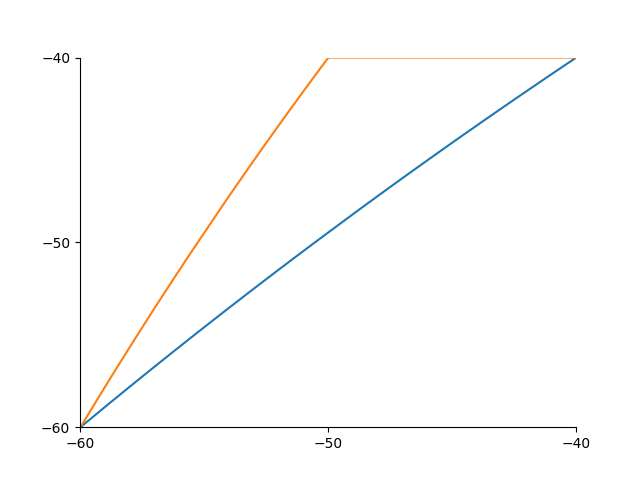
\includegraphics[width=3in]{lit_review/FigAdd} &
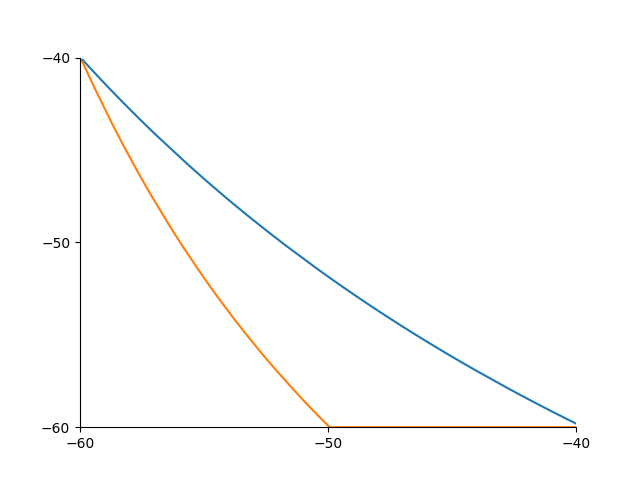
\includegraphics[width=3in]{lit_review/FigSub} \\
(a) Addition & (b) Subtraction \\
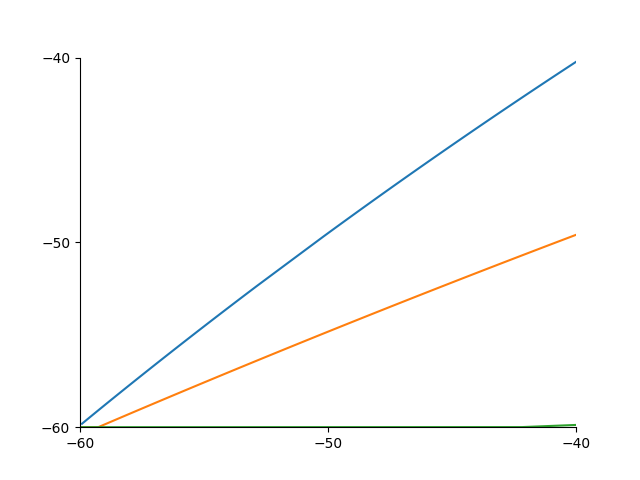
\includegraphics[width=3in]{lit_review/FigMul} &
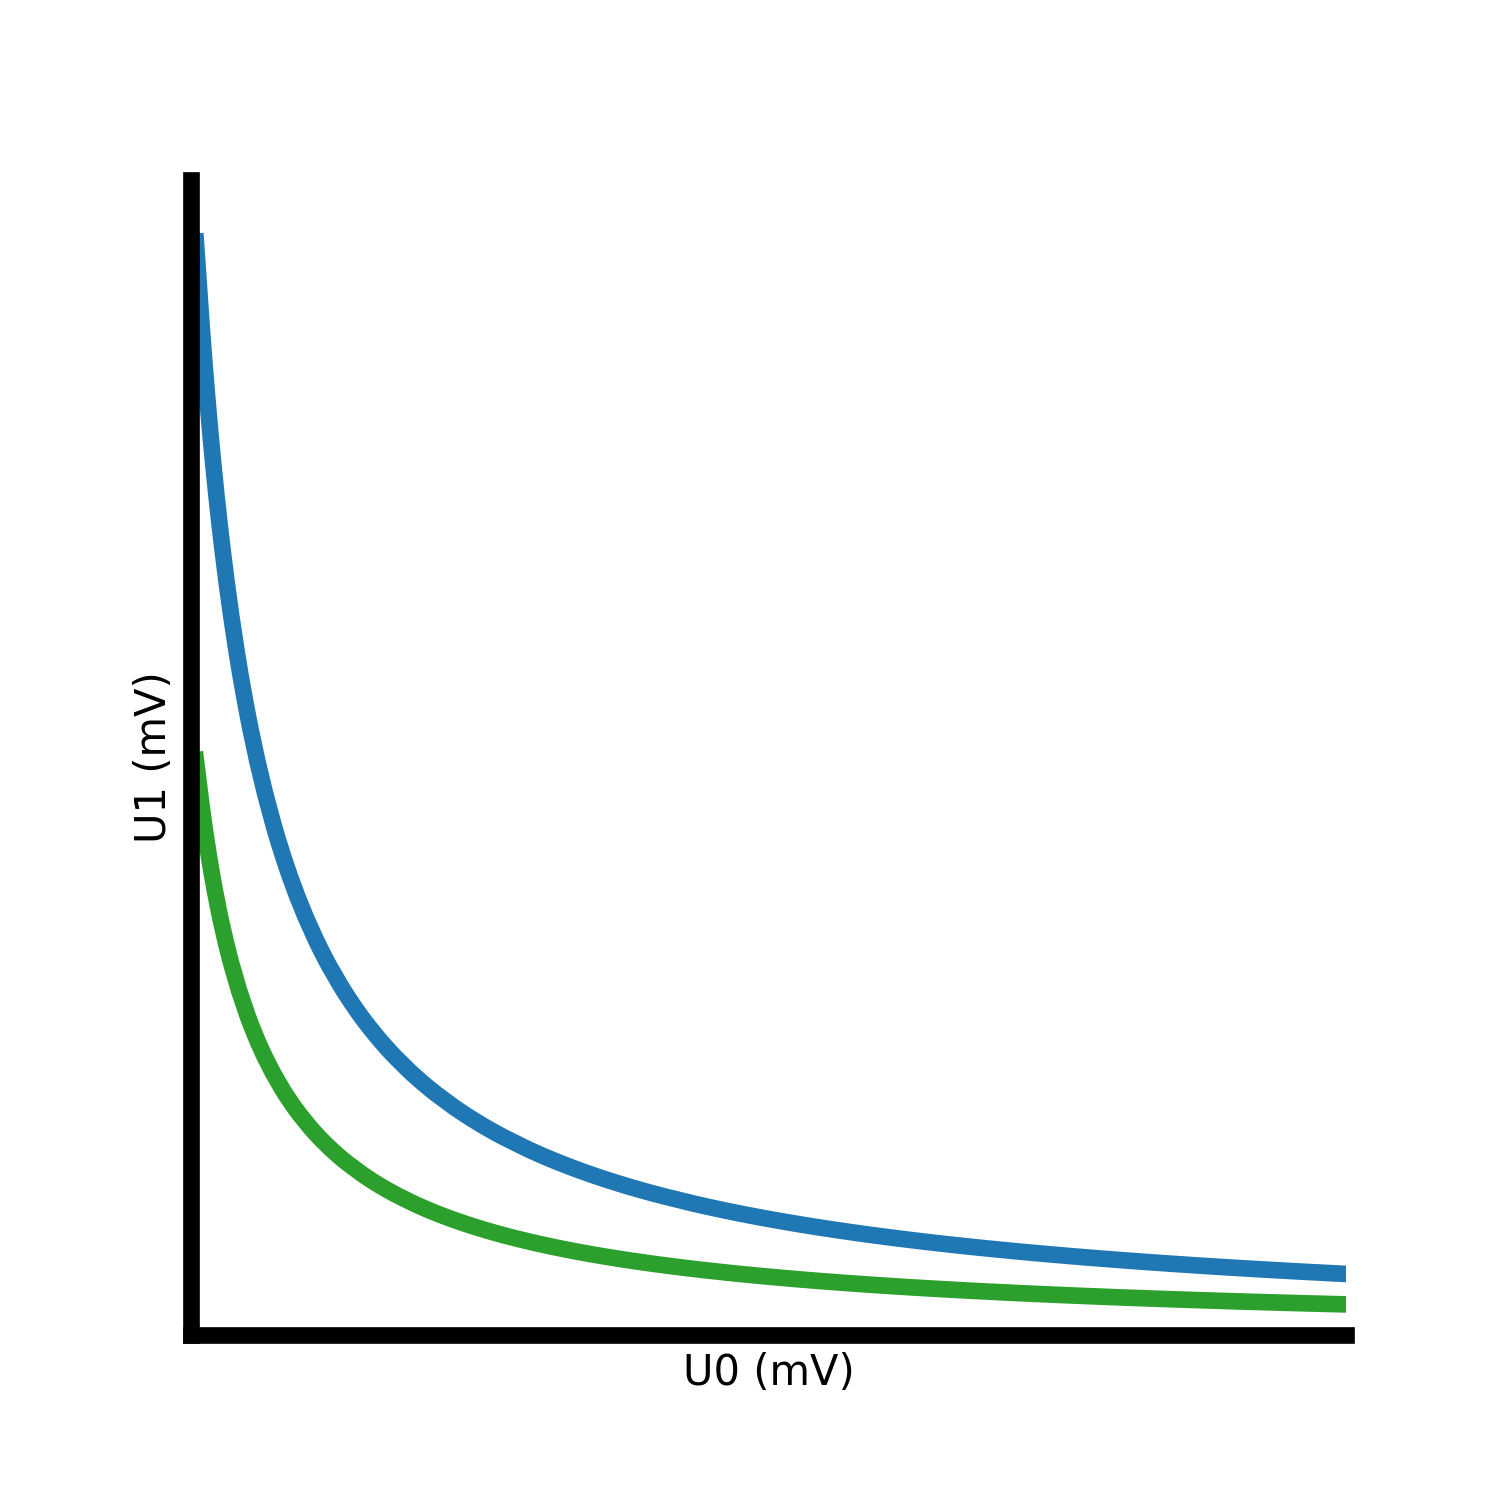
\includegraphics[width=3in]{lit_review/FigDiv} \\
(c) Multiplication & (d) Division \\
\end{tabular}
\caption{Neuron outputs tuned to arithmetic operations adapted from \cite{NickFunctionalSubnetwork}}
\label{fig:MathOutputs}
\end{figure}

These subnetworks can be recursively combined to form larger and more intricate
networks that form a controller. This approach allows for the integration of
existing work in controller design with biological inspiration to increase the
effectiveness of the controller when controlling a biologically inspired robot.
This approach also allows for rapid testing and developing new hypotheses about the underlying function of biological systems in a way that typical controller designs do not.
